\subsection{Fundamentale Verteilungen}

Die größe Untergrundquelle sind nach der vollständigen Selektion die $t\bar{t}$-Prozesse.
Um ihre Eigenschaften besser verstehen zu können, wurden einige Größen hier aufgetragen.
Diese werden dann mit den Erwartungen für $t\bar{t}$-Prozesse verglichen.
Dabei handelt es sich um Monte-Carlo Simulationen des $t\bar{t}$-Prozesses mit Myonen.
Einige dieser Größen sind in Abbildung \ref{fig:Distributions} dargestellt.
Der Rest ist im Anhang in Kapitel \ref{sec:reste} in Abbildung \ref{fig:Distributions2} - \ref{fig:Distributions4} zu finden.
Sie stimmen mit den Erwartungen an den $t\bar{t}$-Prozess gut überein.
So ist zum Biepiel in Abbildung \ref{fig:btagged} die Anzahl an btagged Jets zu sehen.
Btagged Jets sind Jets die mit einer gewissen Wahrscheinlichkeit ($MV1 > 0.7892$) ihren Ursprung in einem b-Quark nahmen.
Da in einem $t\bar{t}$-Prozess, wie in Abbildung \ref{fig:gluonfusion} zu sehen, zwei b-Jets erzeugt werden, ist die Vertilung in er Hinsicht wi zu erwarten.
Der restliche transversale Impuls wird dann gleichermaßen auf das Myon und das Neutrino aufgeteilt.
Diese beiden Verteilungen in Abbildung \ref{fig:lep_pt} und \ref{fig:met_et} weisen einen ähnlichen Peak und Verlauf auf.
Allerdings ist die Verteilung durch die fehlende Auflösung für die Neutrinos etwas ausgeschmierter, bzw. flacher.

\begin{figure}
  \begin{subfigure}{0.5\textwidth}
    \centering
    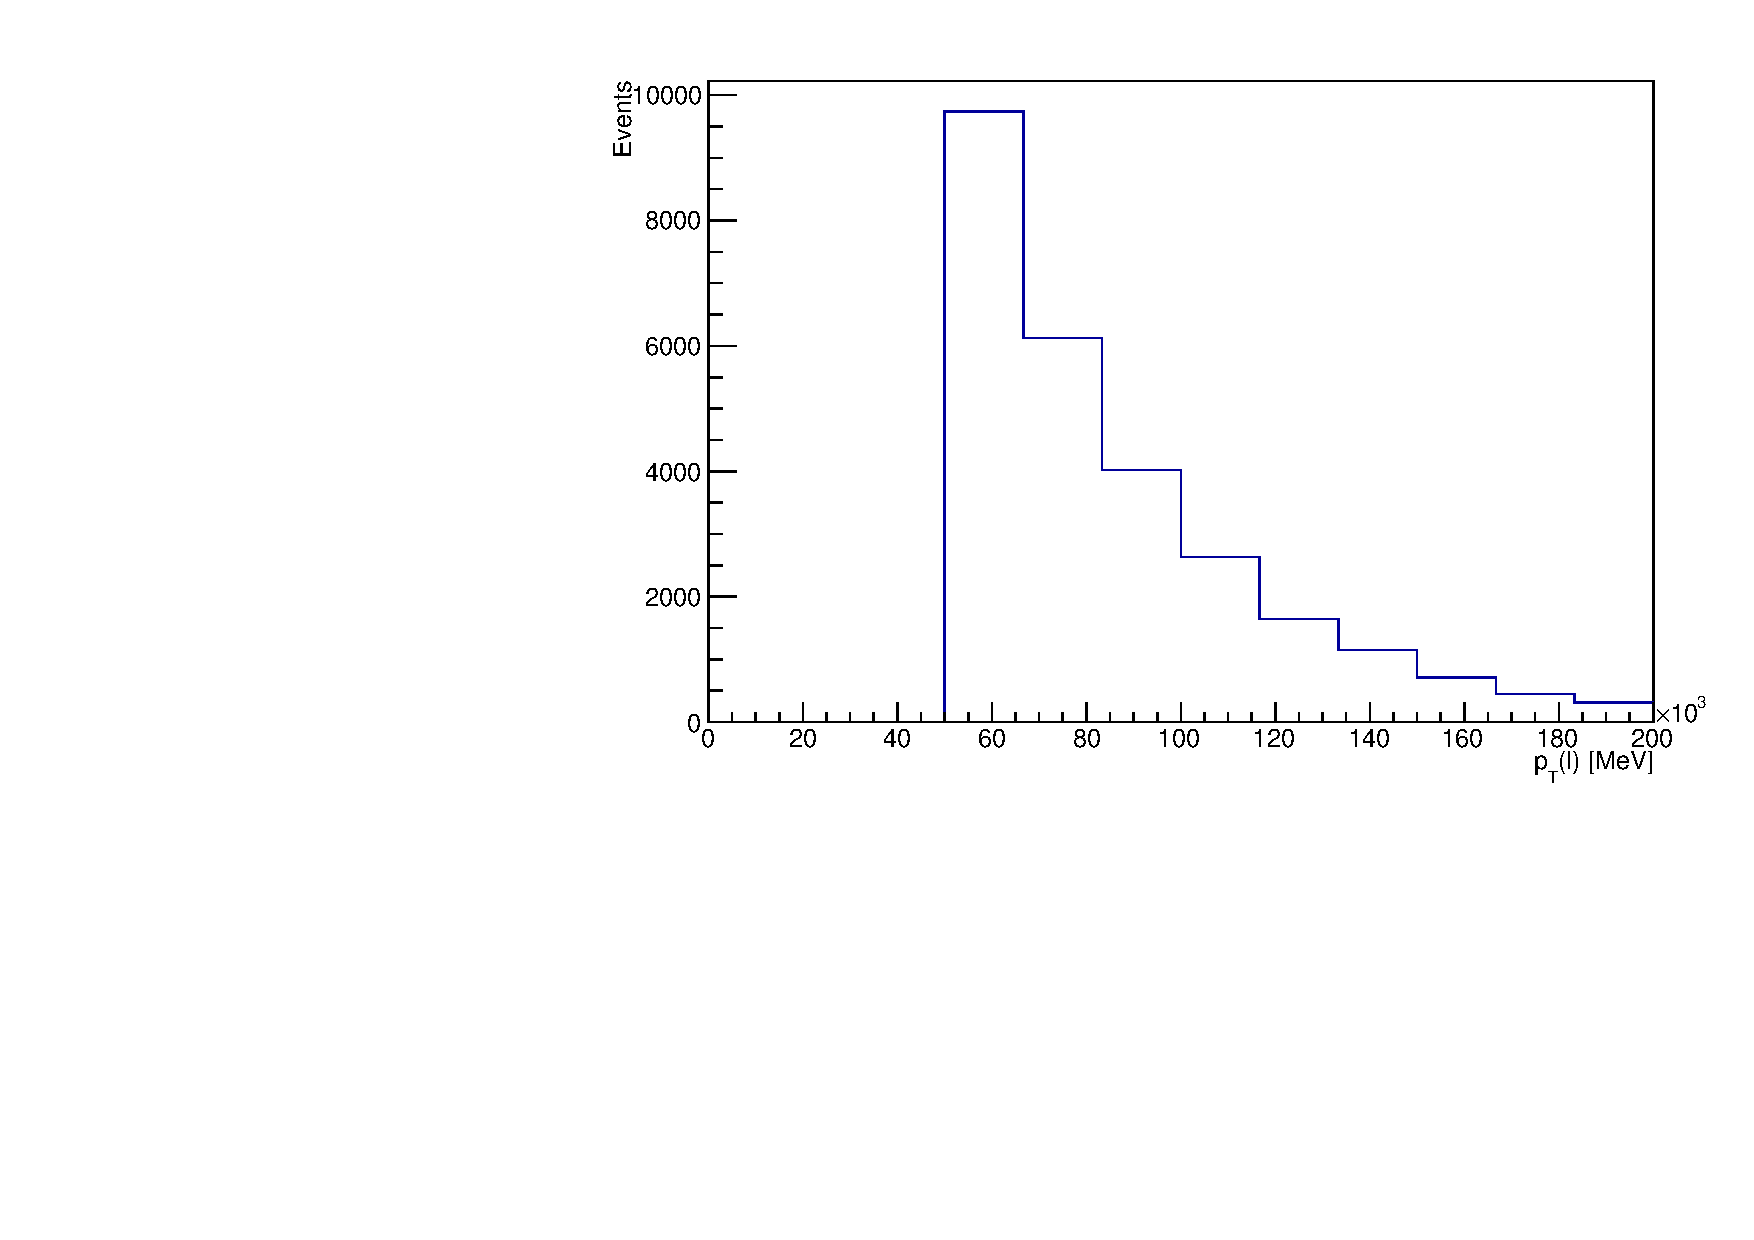
\includegraphics[width=\linewidth]{plots_and_txt/ttbar.mu_selected_/ttbar.mu_selected_lep_pt.pdf}
    \caption{}
    \label{fig:lep_pt}
  \end{subfigure}%
  \begin{subfigure}{0.5\textwidth}
    \centering
    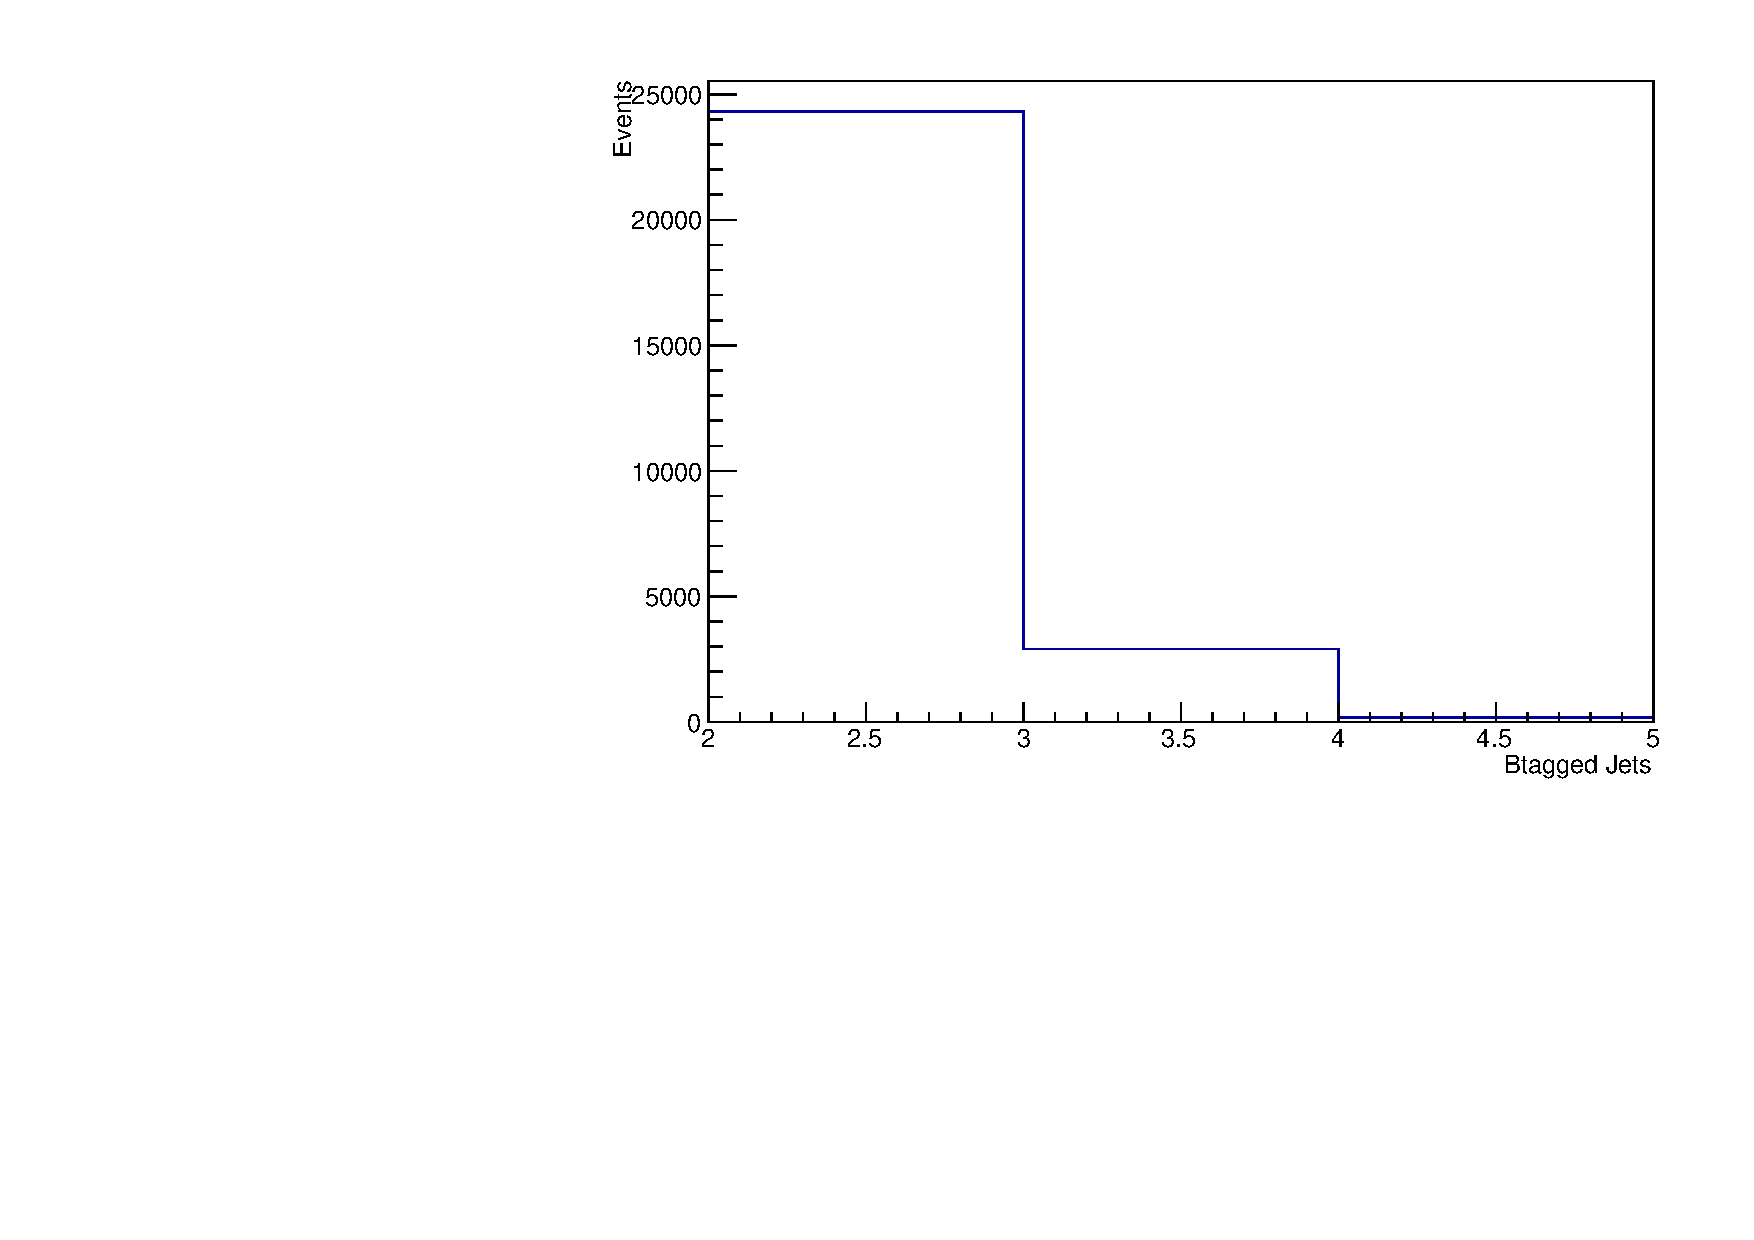
\includegraphics[width=\linewidth]{plots_and_txt/ttbar.mu_selected_/ttbar.mu_selected_btagged.pdf}
    \caption{}
    \label{fig:btagged}
  \end{subfigure}%
  \newline
  \begin{subfigure}{0.5\textwidth}
    \centering
    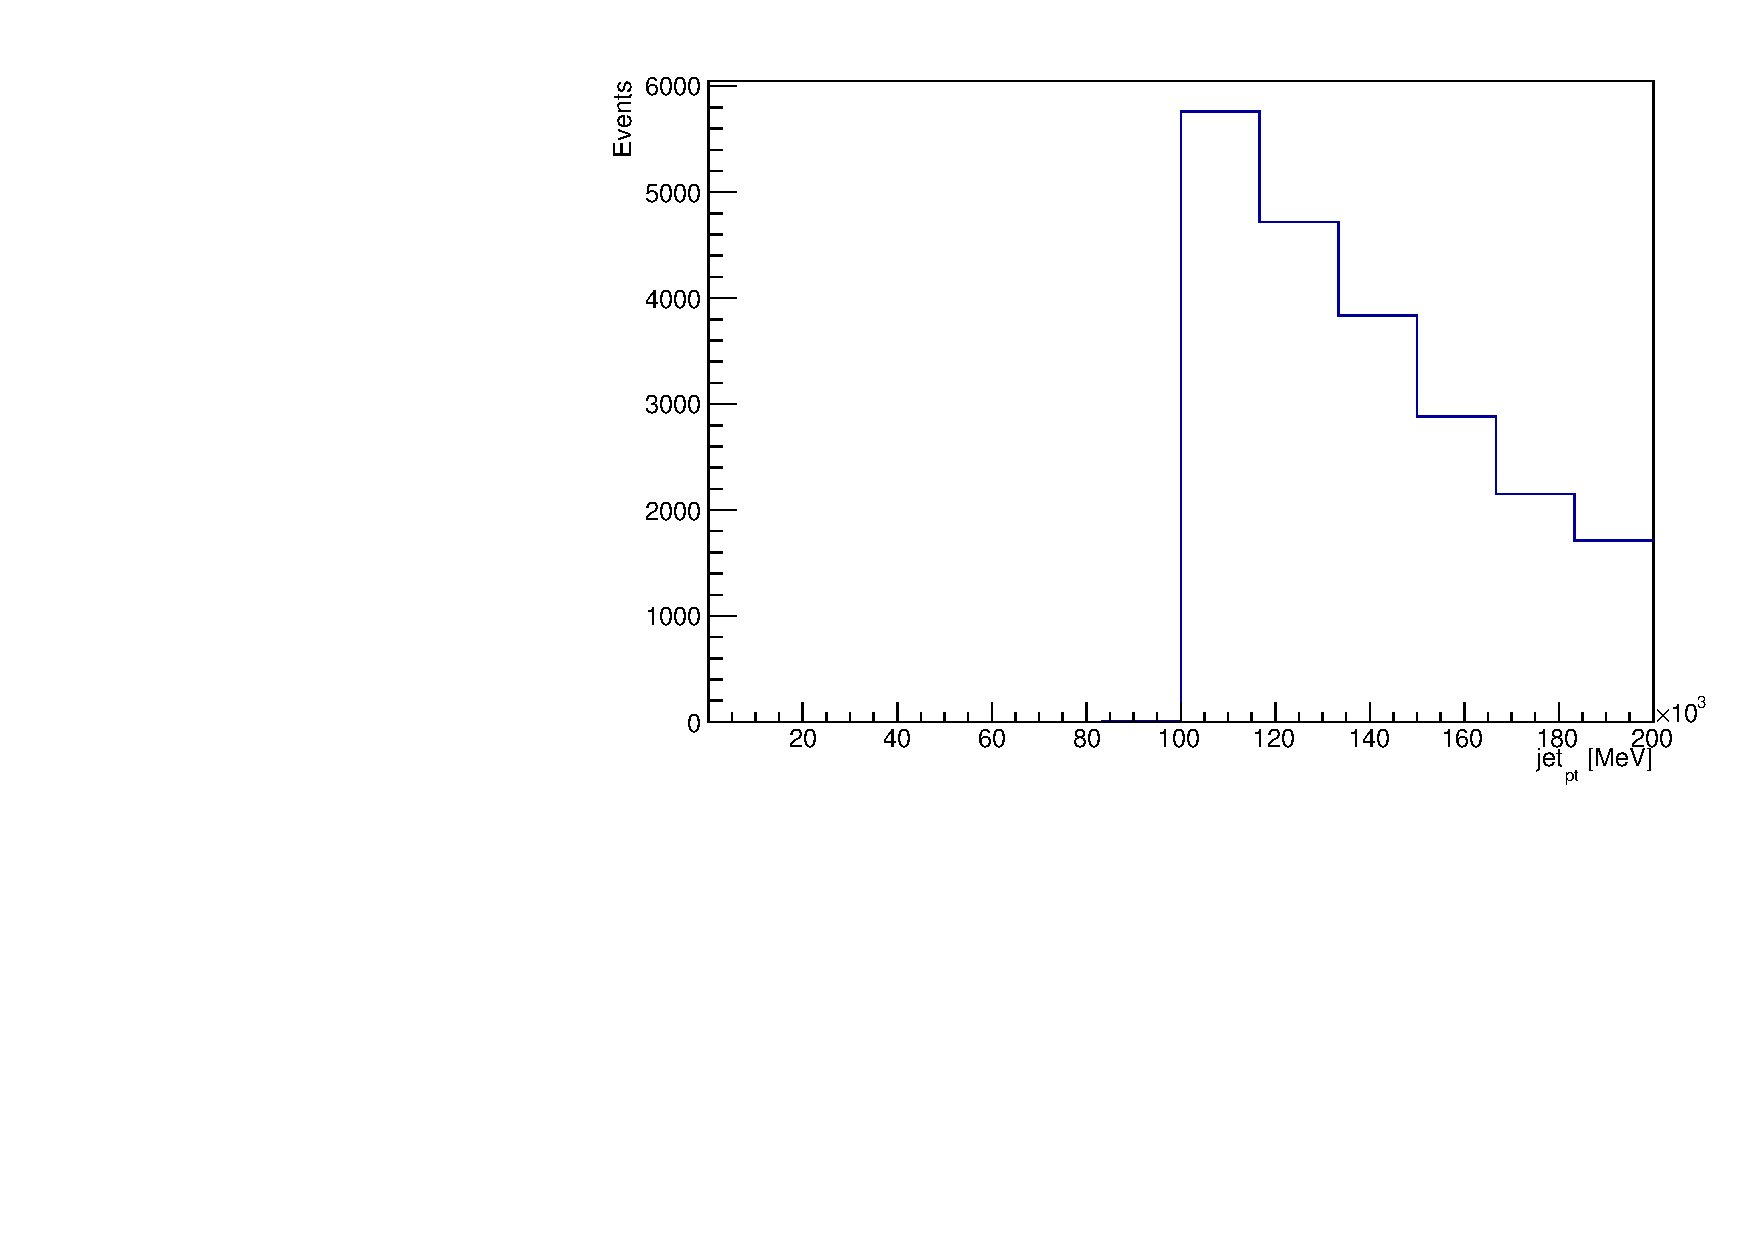
\includegraphics[width=\linewidth]{plots_and_txt/ttbar.mu_selected_/ttbar.mu_selected_jet_pt.pdf}
    \caption{}
    \label{fig:jet_pt_good}
  \end{subfigure}%
  \begin{subfigure}{0.5\textwidth}
    \centering
    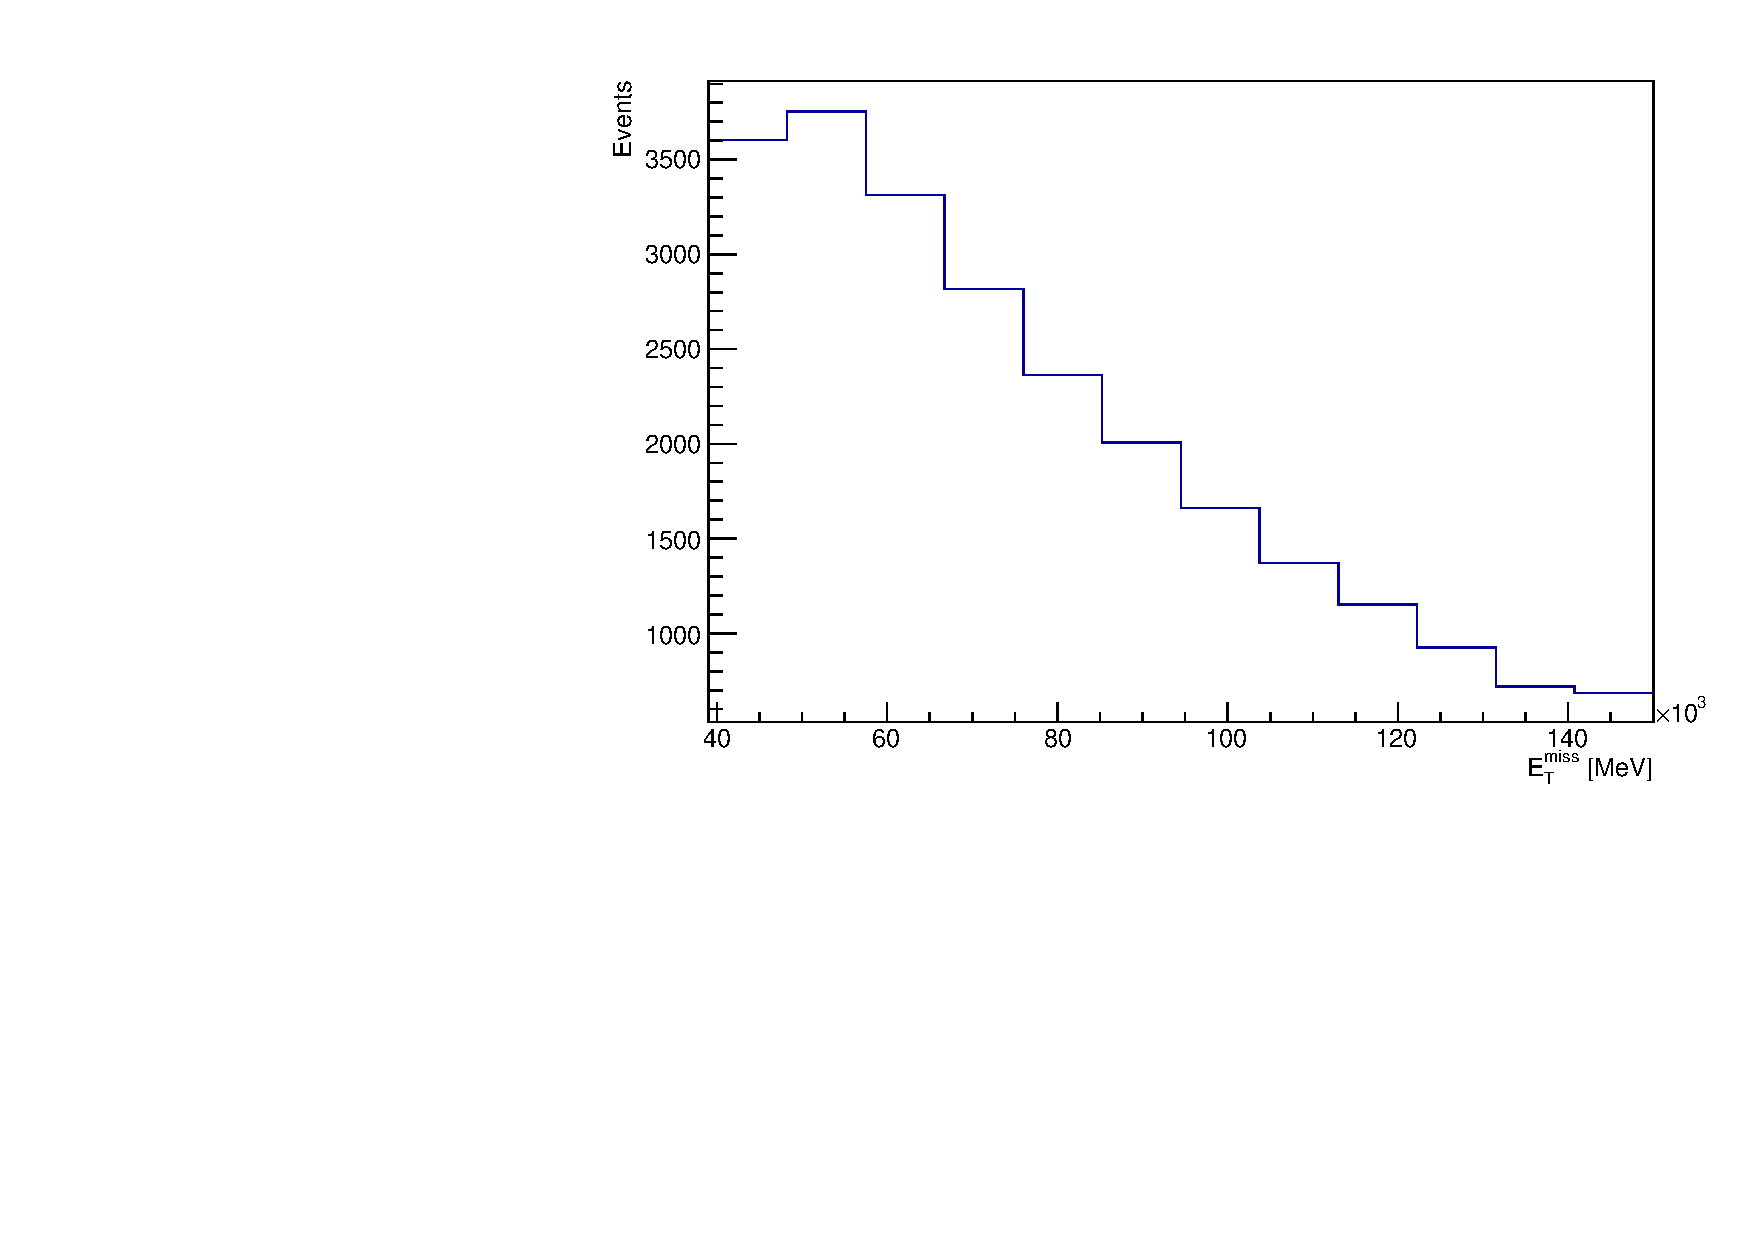
\includegraphics[width=\linewidth]{plots_and_txt/ttbar.mu_selected_/ttbar.mu_selected_met_et.pdf}
    \caption{}
    \label{fig:met_et}
  \end{subfigure}%
  \caption{Darstellung verschiedener Verteilungen der Größen der $t\bar{t}$ Monte-Carlo Simulation.
  Zusehen sind der transverale Impuls der Myonen (\subref{fig:lep_pt}), die Anzahl an btagged Jets (\subref{fig:btagged}), der transverase Impuls des Jets mit dem höchsten transversalen Impuls des Events (\subref{fig:jet_pt_good}) und die fehlende transversal Energie (\subref{fig:met_et}).
  }
  \label{fig:Distributions}
\end{figure}

Auch nach der oben durchgeführten Selektion bleiben Untergrundprozesse wie der hier untersuchte $t\bar{t}$-Prozess übrig.
Um nun eine bessere Unterscheidung zwischen Signalereignissen, also $Z^\prime$-Ereignissen, und den Untergründen herzustellen werden weitere Größen konstruiert.
Da diese unter Umständen mehr Informationen als einfache Größen enthalten, kann ihre Diskriminierungsstärke deutlich erhöht sein.
Untersucht wurden $\Delta\Phi$, die Differenz zwischen dem Azimuthalwinkel der fehlenden Transversalenergie und der Leptonflugrichtung, die invariante Masse des Systems, die durch die drei Jets mit dem größten $p_T$ gebildet wird, die invariante Masse und die Pseudorapidität des Systems, die durch die vier Jets mit dem größten $p_T$, dem Lepton und dem Neutrino gebildet werden.
Für $\Delta\Phi$ wird darauf geachtet, dass jeweils die kleinere Differenz von $|\phi_1 - \phi_2|$ und $|2\pi - |\phi_1 - \phi_2||$ genutzt wird.
Diese werden für alle Datentupel und Monte-Carlo Simulationen berechnet.
Um die Größe mit der stärksten Diskriminierungsstärke zu ermitteln, werden die Verteilungen für den größten Untergrundprozess ($t\bar{t}$) mit einer möglichen Signalverteilung ($Z^\prime(1000)$, also einem hypothetischen $Z^\prime$ mit einer Masse von $\SI{1000}{\giga\electronvolt}$) verglichen.
Dies ist für die nachher gewählte Diskriminante, der vollständigen invarianten Masse des Systems, hier dargestellt.
Die restlichen Vergleiche sind im Anhang in Kapitel \ref{sec:reste} in Abbildung \ref{fig:Comparison1} - \ref{fig:Comparison3} zu sehen.

\begin{figure}
  \begin{subfigure}{0.5\textwidth}
    \centering
    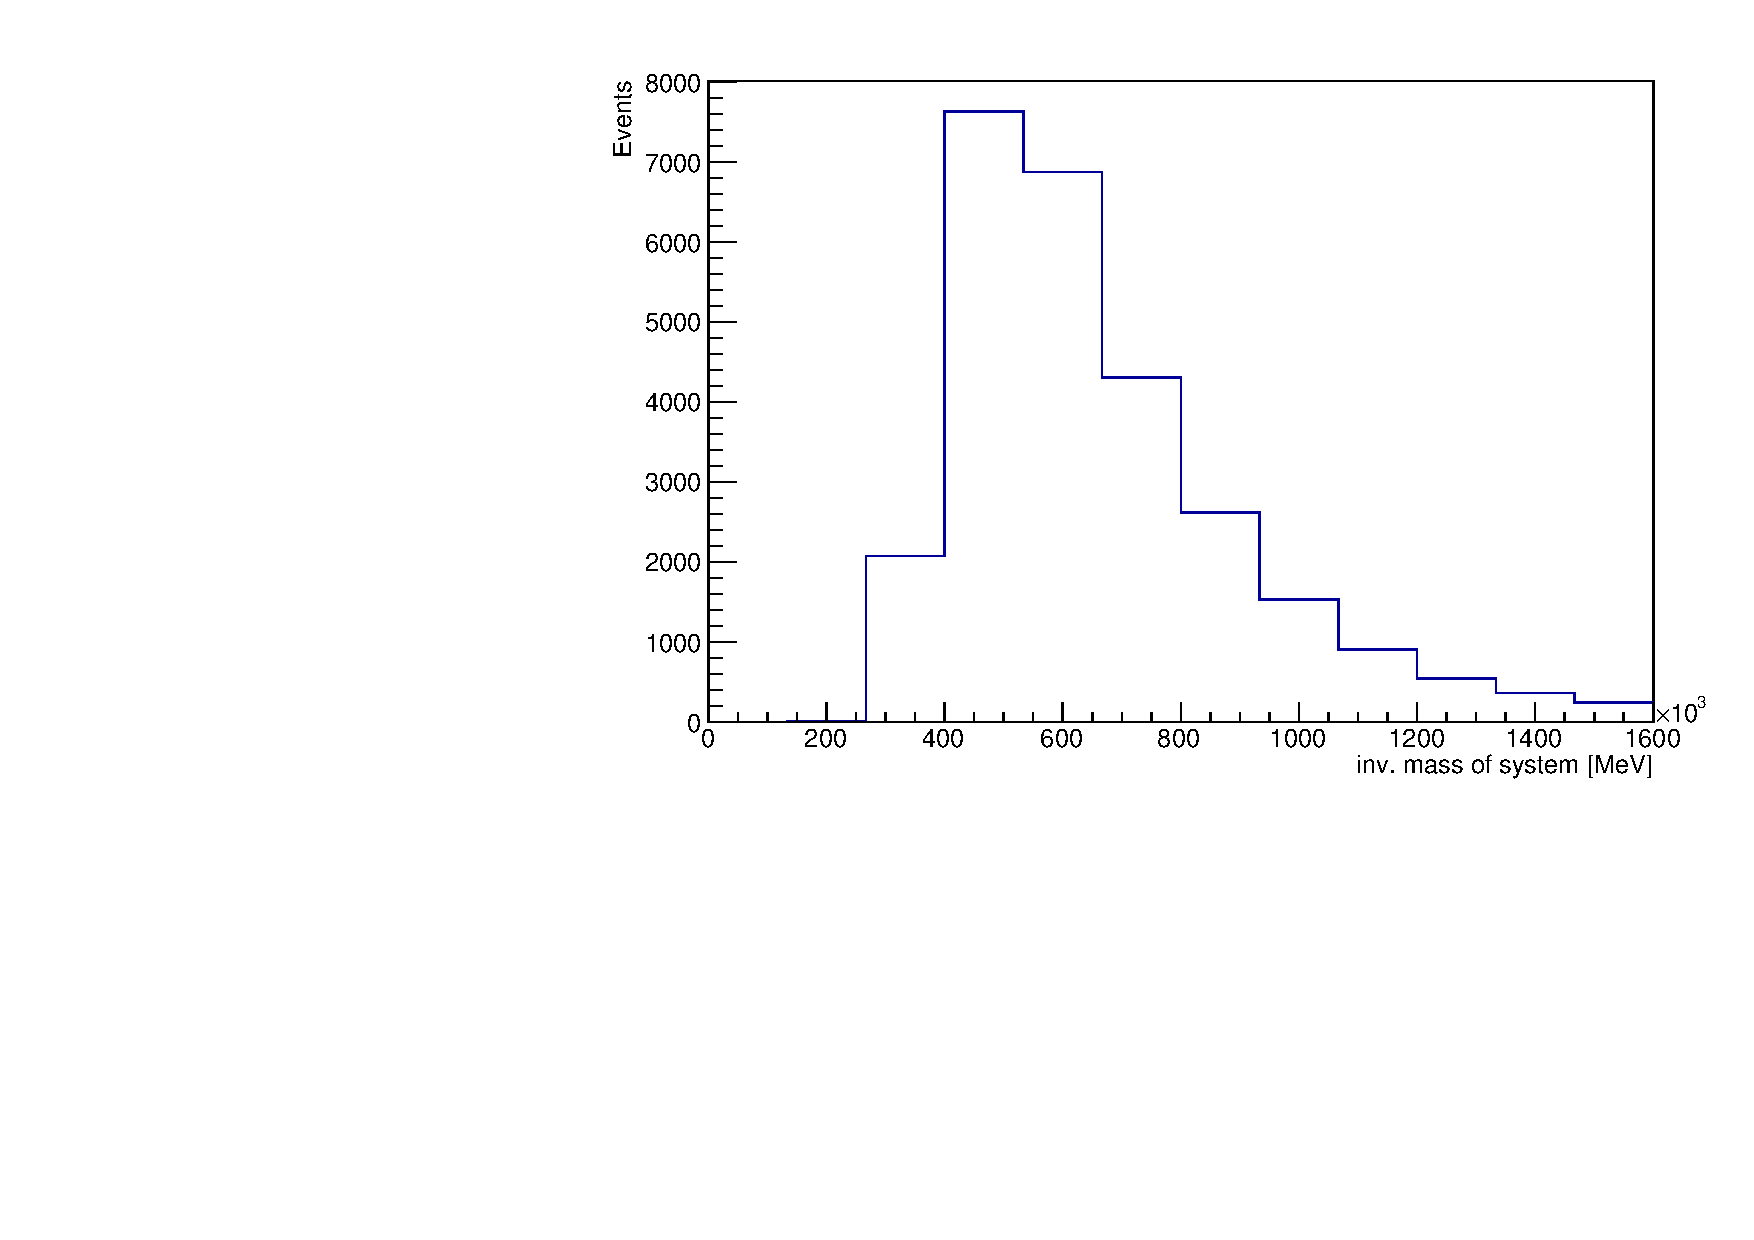
\includegraphics[width=\linewidth]{plots_and_txt/ttbar.mu_selected_/ttbar.mu_selected_SysJetMass.pdf}
    \caption{}
    \label{fig:ttbar_sys}
  \end{subfigure}%
  \begin{subfigure}{0.5\textwidth}
    \centering
    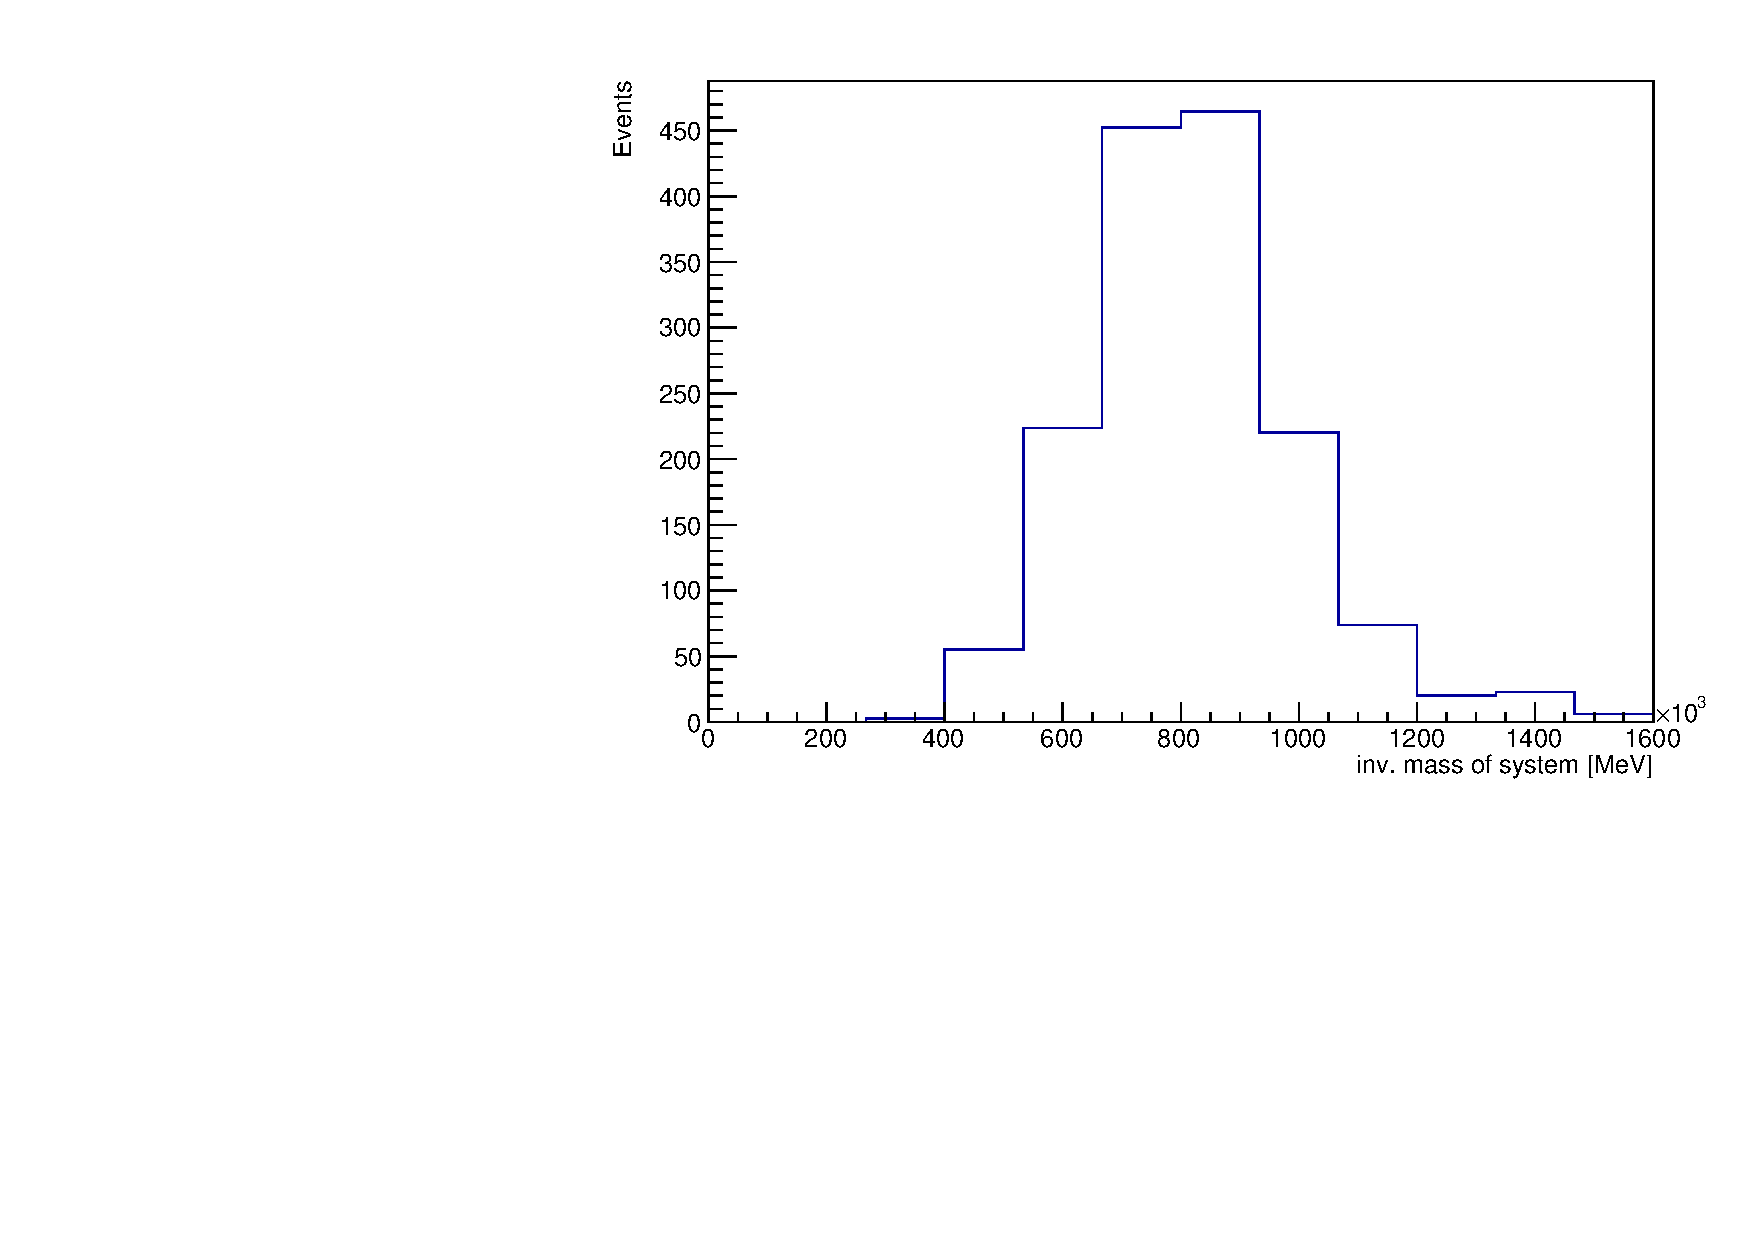
\includegraphics[width=\linewidth]{plots_and_txt/zprime1000.mu_selected_/zprime1000.mu_selected_SysJetMass.pdf}
    \caption{}
    \label{fig:zprime_sys}
  \end{subfigure}%
  \caption{Vergleich der Verteilung der invarianten Masse des Systems, welches aus den vier Jets mit dem größten $p_T$, dem Lepton und dem Neutrino gebildet wird.
  Dies ist für die $t\bar{t}$-Untergrundsimulation \subref{fig:ttbar_sys} und der Signalsimulation des $Z^\prime(1000)$ \subref{fig:zprime_sys} dargestellt.
  Diese Größe dient weiter als Diskriminante.
  }
  \label{fig:Comparison}
\end{figure}













%-
